\documentclass[12pt,letterpaper]{article}
\usepackage{graphicx,textcomp}
\usepackage{natbib}
\usepackage{setspace}
\usepackage{fullpage}
\usepackage{color}
\usepackage[reqno]{amsmath}
\usepackage{amsthm}
\usepackage{fancyvrb}
\usepackage{amssymb,enumerate}
\usepackage[all]{xy}
\usepackage{endnotes}
\usepackage{lscape}
\newtheorem{com}{Comment}
\usepackage{float}
\usepackage{hyperref}
\newtheorem{lem} {Lemma}
\newtheorem{prop}{Proposition}
\newtheorem{thm}{Theorem}
\newtheorem{defn}{Definition}
\newtheorem{cor}{Corollary}
\newtheorem{obs}{Observation}
\usepackage[compact]{titlesec}
\usepackage{dcolumn}
\usepackage{tikz}
\usetikzlibrary{arrows}
\usepackage{multirow}
\usepackage{xcolor}
\newcolumntype{.}{D{.}{.}{-1}}
\newcolumntype{d}[1]{D{.}{.}{#1}}
\definecolor{light-gray}{gray}{0.65}
\usepackage{url}
\usepackage{listings}
\usepackage{color}
\usepackage[utf8]{inputenc}
\usepackage{verbatim} % includes comment blocks
%\usepackage{rotating}
%\usepackage{geometry}
%\usepackage{pdflscape}
\usepackage{lscape}

\definecolor{codegreen}{rgb}{0,0.6,0}
\definecolor{codegray}{rgb}{0.5,0.5,0.5}
\definecolor{codepurple}{rgb}{0.58,0,0.82}
\definecolor{backcolour}{rgb}{0.95,0.95,0.92}

\lstdefinestyle{mystyle}{
	backgroundcolor=\color{backcolour},
	commentstyle=\color{codegreen},
	keywordstyle=\color{magenta},
	numberstyle=\tiny\color{codegray},
	stringstyle=\color{codepurple},
	basicstyle=\footnotesize,
	breakatwhitespace=false,
	breaklines=true,
	captionpos=b,
	keepspaces=true,
	numbers=left,
	numbersep=5pt,
	showspaces=false,
	showstringspaces=false,
	showtabs=false,
	tabsize=2
}
\lstset{style=mystyle}
\newcommand{\Sref}[1]{Section~\ref{#1}}
\newtheorem{hyp}{Hypothesis}

\title{Applied Stats II - Problem Set 1}
\date{Due: March 26, 2023}
\author{Imelda Finn (22334657)}

\begin{document}
	\maketitle
\begin{comment}
	\section*{Instructions}
	\begin{itemize}
	\item Please show your work! You may lose points by simply writing in the answer. If the problem requires you to execute commands in \texttt{R}, please include the code you used to get your answers. Please also include the \texttt{.R} file that contains your code. If you are not sure if work needs to be shown for a particular problem, please ask.
\item Your homework should be submitted electronically on GitHub in \texttt{.pdf} form.
\item This problem set is due before 23:59 on Sunday March 26, 2023. No late assignments will be accepted.
	\end{itemize}

	\vspace{.25cm}
\end{comment}

	Code in \texttt{PS3\_ImeldaFinn.R}

\section*{Question 1}
\vspace{.25cm}
\noindent We are interested in how governments' management of public resources impacts economic prosperity. Our data come from \href{https://www.researchgate.net/profile/Adam_Przeworski/publication/240357392_Classifying_Political_Regimes/links/0deec532194849aefa000000/Classifying-Political-Regimes.pdf}{Alvarez, Cheibub, Limongi, and Przeworski (1996)} and is labelled \texttt{gdpChange.csv} on GitHub. The dataset covers 135 countries observed between 1950 or the year of independence or the first year forwhich data on economic growth are available (``entry year"), and 1990 or the last year for which data on economic growth are available (``exit year"). The unit of analysis is a particular country during a particular year, for a total $>$ 3,500 observations. 

\begin{itemize}
	\item
	Response variable: 
	\begin{itemize}
		\item \texttt{GDPWdiff}: Difference in GDP between year $t$ and $t-1$. Possible categories include: ``positive", ``negative", or ``no change"
	\end{itemize}
	\item
	Explanatory variables: 
	\begin{itemize}
		\item
		\texttt{REG}: 1=Democracy; 0=Non-Democracy
		\item
		\texttt{OIL}: 1=if the average ratio of fuel exports to total exports in 1984-86 exceeded 50\%; 0= otherwise
	\end{itemize}
	
\end{itemize}

  The data was read in and \texttt{GDPWDiff} was factored.  The cutoff point was 0, ie values less than 0 were categorised as \emph{negative}, values equal to 0 were categorised as \emph{no change} and values above 0 were categorised as \emph{positive}.  \emph{no change} was set as the reference category.
  %64-67
  \lstinputlisting[language=R, firstline=64, lastline=68]{PS3_ImeldaFinn.R}
  %===============================================================
  \begin{comment}
  \begin{lstlisting}[language=R]
      gdp <- read_csv("./data/gdpChange.csv")
      gdp$diff <- ifelse(gdp$GDPWdiff==0, "no change", 
                   ifelse(gdp$GDPWdiff>0, "positive", "negative")) 
      gdp$diff2 <- relevel(factor(gdp$diff, ordered = FALSE), ref="no change")
  \end{lstlisting}

  \begin{sidewaystable}
%\begin{tabular}...\end{tabular}
  \end{sidewaystable}
  %
% Table created by stargazer v.5.2.3 by Marek Hlavac, Social Policy Institute. E-mail: marek.hlavac at gmail.com
% Date and time: Tue, Mar 21, 2023 - 15:08:02
\begin{table}[!htbp] \centering 
  \caption{} 
  \label{tbl:gdp} 
\begin{tabular}{@{\extracolsep{5pt}} ccccccc} 
\\[-1.8ex]\hline 
\hline \\[-1.8ex] 
GDPWdiff & GDPWdiff & Min / Max & -2506.0 / 2821.0 & -3741.0 / 3722.0 & -9257.0 / 7867.0 & -5997.0 / 3555.0 \\ 
GDPWdiff & GDPWdiff & Med [IQR] & 50.0 [-30.0;215.0] & 293.0 [13.5;644.8] & 140.5 [-50.0;463.0] & 39.0 [-527.2;421.8] \\ 
GDPWdiff & GDPWdiff & Mean (std) & 106.0 (395.3) & 319.4 (561.6) & 141.2 (1147.3) & -46.5 (1228.4) \\ 
GDPWdiff & GDPWdiff & N (NA) & 1939 (0) & 1408 (0) & 288 (0) & 86 (0) \\ 
\hline \\[-1.8ex] 
\end{tabular} 
\end{table} 

% Table created by stargazer v.5.2.3 by Marek Hlavac, Social Policy Institute. E-mail: marek.hlavac at gmail.com
% Date and time: Tue, Mar 21, 2023 - 15:08:02
\begin{table}[!htbp] \centering 
  \caption{} 
  \label{tbl:gdp} 
\begin{tabular}{@{\extracolsep{5pt}} c} 
\\[-1.8ex]\hline 
\hline \\[-1.8ex] 
GDP data summary \\ 
\hline \\[-1.8ex] 
\end{tabular} 
\end{table}  


  \begin{landscape}
    
% Table created by stargazer v.5.2.3 by Marek Hlavac, Social Policy Institute. E-mail: marek.hlavac at gmail.com
% Date and time: Tue, Mar 21, 2023 - 15:08:02
\begin{table}[!htbp] \centering 
  \caption{} 
  \label{tbl:gdp} 
\begin{tabular}{@{\extracolsep{5pt}} ccccccc} 
\\[-1.8ex]\hline 
\hline \\[-1.8ex] 
GDPWdiff & GDPWdiff & Min / Max & -2506.0 / 2821.0 & -3741.0 / 3722.0 & -9257.0 / 7867.0 & -5997.0 / 3555.0 \\ 
GDPWdiff & GDPWdiff & Med [IQR] & 50.0 [-30.0;215.0] & 293.0 [13.5;644.8] & 140.5 [-50.0;463.0] & 39.0 [-527.2;421.8] \\ 
GDPWdiff & GDPWdiff & Mean (std) & 106.0 (395.3) & 319.4 (561.6) & 141.2 (1147.3) & -46.5 (1228.4) \\ 
GDPWdiff & GDPWdiff & N (NA) & 1939 (0) & 1408 (0) & 288 (0) & 86 (0) \\ 
\hline \\[-1.8ex] 
\end{tabular} 
\end{table} 

% Table created by stargazer v.5.2.3 by Marek Hlavac, Social Policy Institute. E-mail: marek.hlavac at gmail.com
% Date and time: Tue, Mar 21, 2023 - 15:08:02
\begin{table}[!htbp] \centering 
  \caption{} 
  \label{tbl:gdp} 
\begin{tabular}{@{\extracolsep{5pt}} c} 
\\[-1.8ex]\hline 
\hline \\[-1.8ex] 
GDP data summary \\ 
\hline \\[-1.8ex] 
\end{tabular} 
\end{table}  

  \end{landscape}

  \end{comment}
  %===============================================================
  \begin{figure}[!htbp]
	  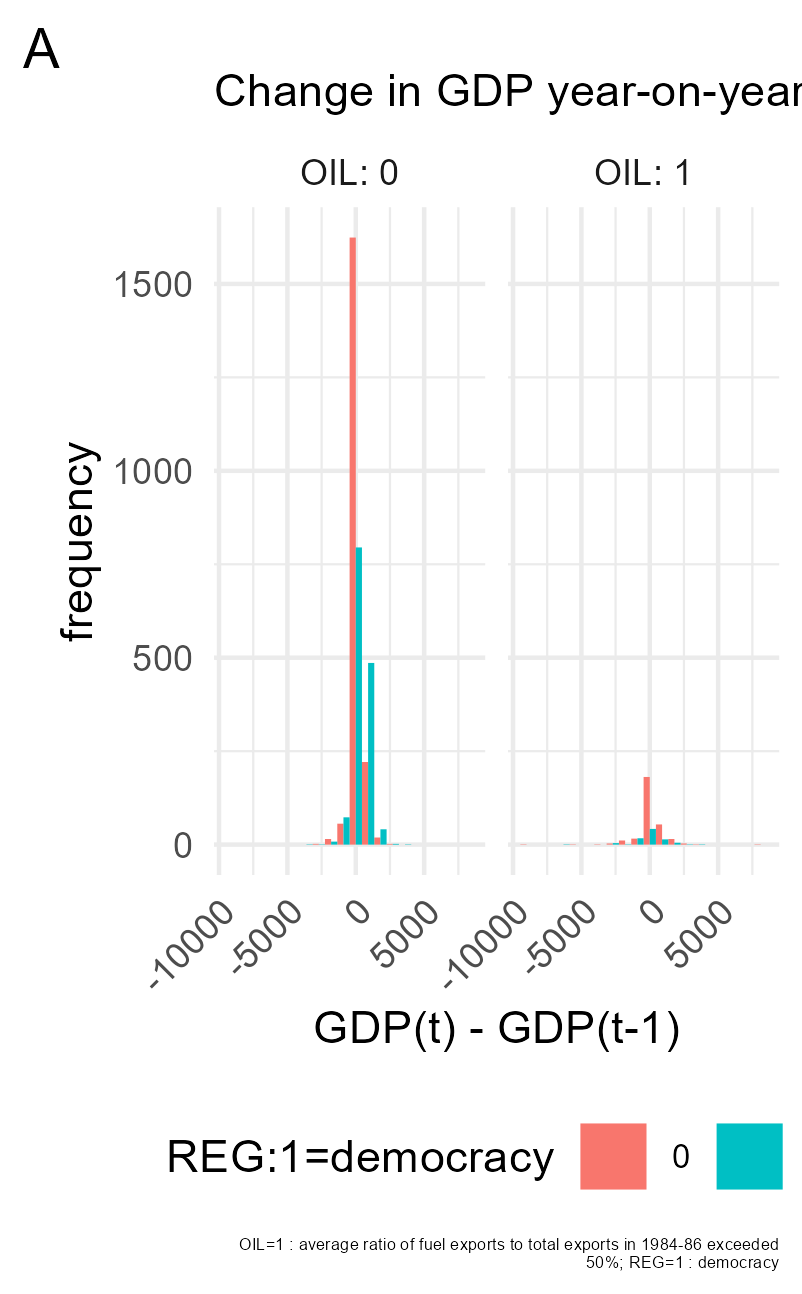
\includegraphics[width=0.7\textwidth]{graphics/gdp_hist.png}
	  %\caption{GDP difference data}
	  %\label{fig:gdp:hist}
%	\end{figure}

%  \begin{figure}[!htbp]
	  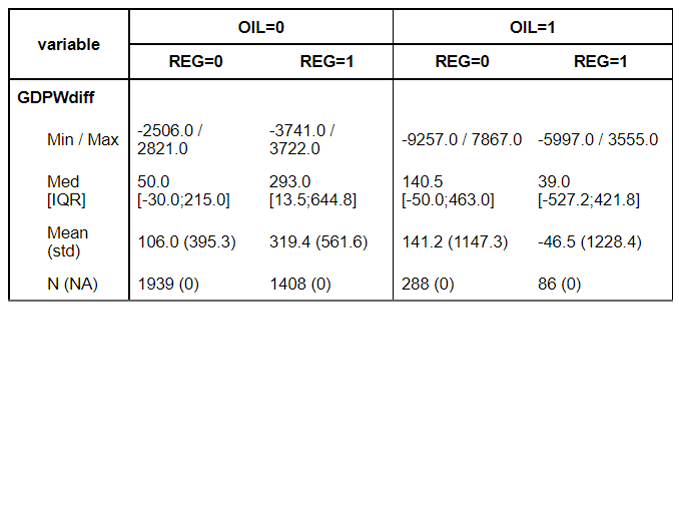
\includegraphics[width=0.7\textwidth]{graphics/gdp_flextab.png}
	  \caption{GDP difference Data}
	  \label{fig:gdp}
	\end{figure}
	\clearpage

%\newpage
%\noindent Please answer the following questions:

\begin{enumerate}
	\item An unordered multinomial logit with \texttt{GDPWdiff} as the output was constructed as follows:
    \lstinputlisting[language=R, firstline=115, lastline=115]{PS3_ImeldaFinn.R}

	The results of the model are shown in Table~\ref{tbl:multinom}.  The predicted probabilities are shown in Table~\ref{tbl:pred:multi}, Figure~\ref{fig:pred:multi}.  All of the predicted classes are $positive$.  This isn't unexpected as Figure~\ref{fig:gdp} shows that the data is skewed towards positive values.
	
  
% Table created by stargazer v.5.2.3 by Marek Hlavac, Social Policy Institute. E-mail: marek.hlavac at gmail.com
% Date and time: Tue, Mar 21, 2023 - 21:23:19
\begin{table}[!htbp] \centering 
  \caption{Multinomial, unordered} 
  \label{tbl:multinom} 
\begin{tabular}{@{\extracolsep{5pt}}lcc} 
\\[-1.8ex]\hline 
\hline \\[-1.8ex] 
 & \multicolumn{2}{c}{\textit{Dependent variable:}} \\ 
\cline{2-3} 
\\[-1.8ex] & negative & positive \\ 
\\[-1.8ex] & (1) & (2)\\ 
\hline \\[-1.8ex] 
 REG & 1.379 & 1.769 \\ 
  & t = 1.794 & t = 2.306 \\ 
  & p = 0.073$^{*}$ & p = 0.022$^{**}$ \\ 
  & & \\ 
 OIL & 4.784 & 4.576 \\ 
  & t = 0.695 & t = 0.665 \\ 
  & p = 0.488 & p = 0.507 \\ 
  & & \\ 
 Constant & 3.805 & 4.534 \\ 
  & t = 14.058 & t = 16.842 \\ 
  & p = 0.000$^{***}$ & p = 0.000$^{***}$ \\ 
  & & \\ 
\hline \\[-1.8ex] 
Akaike Inf. Crit. & 4,690.770 & 4,690.770 \\ 
\hline 
\hline \\[-1.8ex] 
\textit{Note:}  & \multicolumn{2}{r}{$^{*}$p$<$0.1; $^{**}$p$<$0.05; $^{***}$p$<$0.01} \\ 
\end{tabular} 
\end{table}  


	The baseline category is regime \texttt{REG} = 0 (non-democracy) and \texttt{OIL} = 0 (not a significant oil exporter).  The predicted probability of having no change in GDP when in the baseline category is 0.7\%.

  \begin{lstlisting}[language=R]
  	round(predict(multinom_model, newdata = data.frame(REG=0, OIL=0),
        type = "probs"),2)

    predict_data <- data.frame(REG = rep(c(0,1), each = 2), 
                           OIL= rep(c(0,1), 2))
    cbind(predict_data, predict(multinom_model,
            newdata = predict_data, type = "class"))
  \end{lstlisting}
  \begin{lstlisting}
  no change  negative  positive 
     0.01      0.32      0.67 

 REG OIL predict(multinom_model, newdata = predict_data, type = "class")
1   0   0                                                        positive
2   0   1                                                        positive
3   1   0                                                        positive
4   1   1                                                        positive

            no change negative positive  Sum
  no change         0        0       16   16
  negative          0        0     1105 1105
  positive          0        0     2600 2600
  Sum               0        0     3721 3721
  \end{lstlisting}
	
  
% Table created by stargazer v.5.2.3 by Marek Hlavac, Social Policy Institute. E-mail: marek.hlavac at gmail.com
% Date and time: Tue, Mar 21, 2023 - 21:00:16
\begin{table}[!htbp] \centering 
  \caption{Predicted results from unordered Multinomial} 
  \label{tbl:pred:multi} 
\begin{tabular}{@{\extracolsep{5pt}} ccccc} 
\\[-1.8ex]\hline 
\hline \\[-1.8ex] 
 & REG & OIL & level & probability \\ 
\hline \\[-1.8ex] 
1 & $0$ & $0$ & no change & $0.007$ \\ 
2 & $0$ & $1$ & no change & $0.0001$ \\ 
3 & $1$ & $0$ & no change & $0.001$ \\ 
4 & $1$ & $1$ & no change & $0.00001$ \\ 
5 & $0$ & $0$ & negative & $0.323$ \\ 
6 & $0$ & $1$ & negative & $0.373$ \\ 
7 & $1$ & $0$ & negative & $0.246$ \\ 
8 & $1$ & $1$ & negative & $0.287$ \\ 
9 & $0$ & $0$ & positive & $0.670$ \\ 
10 & $0$ & $1$ & positive & $0.627$ \\ 
11 & $1$ & $0$ & positive & $0.753$ \\ 
12 & $1$ & $1$ & positive & $0.713$ \\ 
\hline \\[-1.8ex] 
\end{tabular} 
\end{table}  


  Holding \texttt{OIL} constant:
  \begin{itemize}
    \item a change in REG from 0 to 1 increases the log-odds of  \texttt{diff}$ = positive$ vs. \texttt{diff} = \emph{no change} by 1.769
    \item a change in REG from 0 to 1 multiplies the odds of \texttt{diff}$ = positive$ vs. \texttt{diff} $= no~change$ by a factor of $e^{1.769} = 5.87$.
  \end{itemize}

  \begin{figure}[!htbp]
	  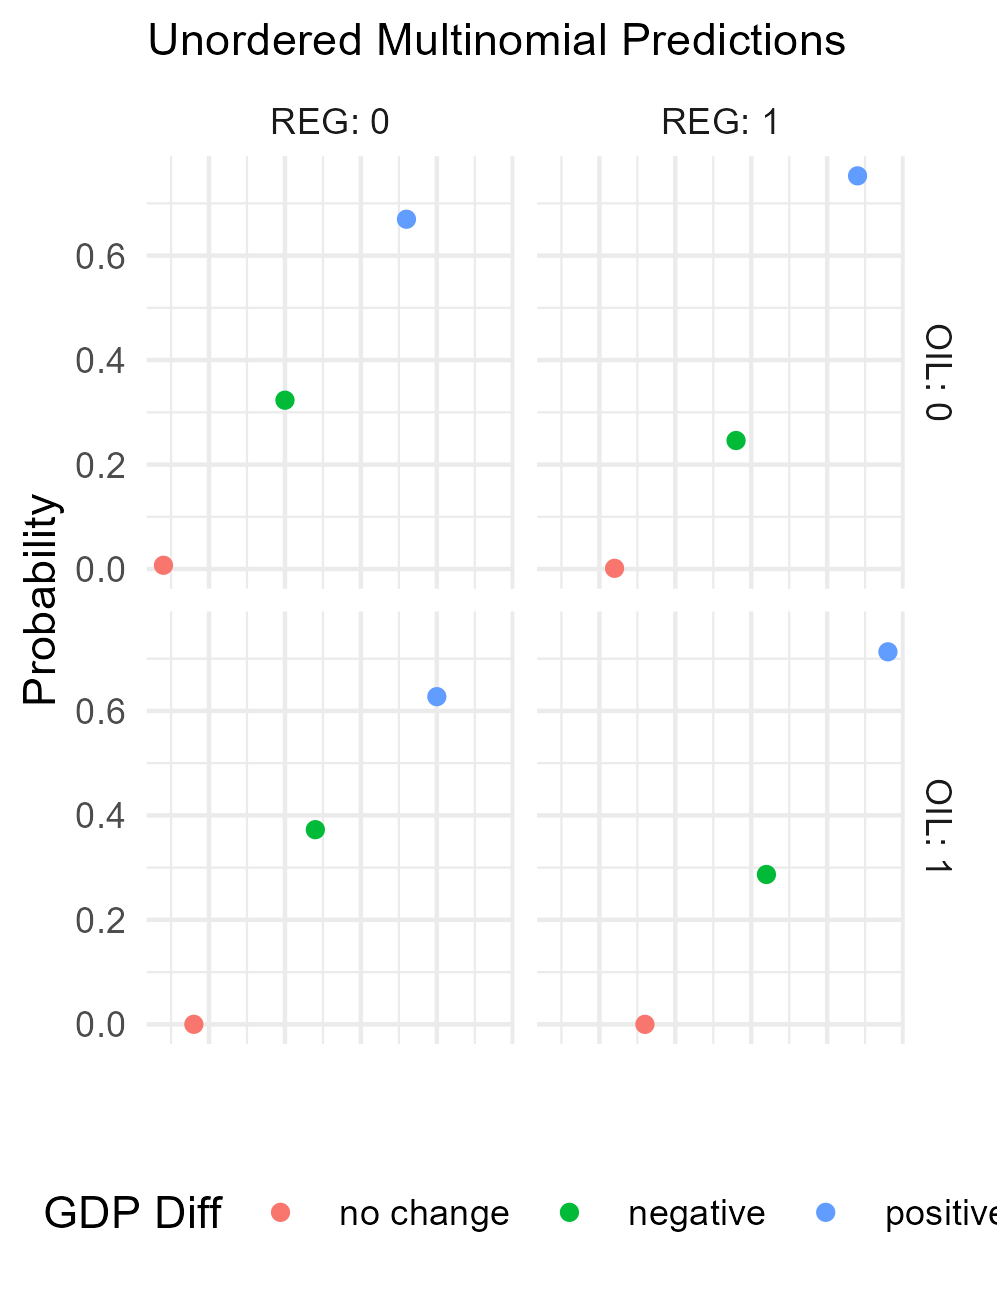
\includegraphics[width=0.7\textwidth]{graphics/pred_multi.png}
	  \caption{GDP Diff - unordered multinomial predictions}
	  \label{fig:pred:multi}
	\end{figure}
	\clearpage

%TODO cutoff 
%---------------------------------------------------------------------
	\item 	The factored \texttt{GDPWdiff} response variable (from 1) was ordered: ($negative<no ~change<positive$), i.e. the cutoff (0) was unchanged.  An ordered multinomial logit model was created as follows:
    \lstinputlisting[language=R, firstline=264, lastline=266]{PS3_ImeldaFinn.R}
    
	The results of the model are shown in Table~\ref{tbl:ordered}.  
	The baseline category is regime \texttt{REG} = 0 (non-democracy) and \texttt{OIL} = 0 (not a significant oil exporter).  The predicted probability of having no change in GDP when in the baseline category is 0.5\% (Table~\ref{tbl:pred:ord}).
	
  
% Table created by stargazer v.5.2.3 by Marek Hlavac, Social Policy Institute. E-mail: marek.hlavac at gmail.com
% Date and time: Tue, Mar 21, 2023 - 21:26:45
\begin{table}[!htbp] \centering 
  \caption{Multinomial Logit, ordered} 
  \label{tbl:ordered} 
\begin{tabular}{@{\extracolsep{5pt}}lc} 
\\[-1.8ex]\hline 
\hline \\[-1.8ex] 
 & \multicolumn{1}{c}{\textit{Dependent variable:}} \\ 
\cline{2-2} 
\\[-1.8ex] & ordered\_diff \\ 
\hline \\[-1.8ex] 
 REG & 0.398 \\ 
  & (0.075) \\ 
  & t = 5.300 \\ 
  & p = 0.00000$^{***}$ \\ 
  & \\ 
 OIL & $-$0.199 \\ 
  & (0.116) \\ 
  & t = $-$1.717 \\ 
  & p = 0.086$^{*}$ \\ 
  & \\ 
 negative\textbar no change & $-$0.731 \\ 
  & (0.048) \\ 
  & t = $-$15.360 \\ 
  & p = 0.000$^{***}$ \\ 
  & \\ 
 no change\textbar positive & $-$0.710 \\ 
  & (0.048) \\ 
  & t = $-$14.955 \\ 
  & p = 0.000$^{***}$ \\ 
  & \\ 
\hline \\[-1.8ex] 
Observations & 3,721 \\ 
\hline 
\hline \\[-1.8ex] 
\textit{Note:}  & \multicolumn{1}{r}{$^{*}$p$<$0.1; $^{**}$p$<$0.05; $^{***}$p$<$0.01} \\ 
\end{tabular} 
\end{table}  


  The coefficients and their confidence intervals are:
  \begin{lstlisting}[language=R]
    cbind(logOdds = coef(ord_model), confint(ord_model))
    #       logOdds      2.5 %     97.5 %
    #REG  0.3984834  0.2516548 0.54643410
    #OIL -0.1987177 -0.4237548 0.03019571
  \end{lstlisting}

  Holding \texttt{REG} constant:
  \begin{itemize}
    \item a change in OIL from 0 to 1 changes the log-odds of  \texttt{diff}$ = no~change$ vs. \texttt{diff} = \emph{negative} by -0.199
    \item a change in OIL from 0 to 1 multiplies the odds of \texttt{diff}$ = no~change$ vs. \texttt{diff} = \emph{negative} by a factor of $e^{-0.199} = 0.82$.
  \end{itemize}

  The odds of having no change in GDP growth for a country that has oil, are .18\% lower compared to a country that doesn't have oil, holding regime status constant.

  \begin{lstlisting}[language=R]
  round(predict(ord_model, newdata = data.frame(REG=0, OIL=0), type = "probs"),2)
  predict(ord_model, newdata = data.frame(REG=0, OIL=0), type = "class")
  cbind(predict_data, predict(ord_model, predict_data, type="class"))
  \end{lstlisting}
  \begin{lstlisting}
 negative no change  positive 
     0.32      0.00      0.67 

[1] positive
Levels: negative no change positive

  REG OIL predict(ord_model, predict_data, type = "class")
1   0   0                                         positive
2   0   1                                         positive
3   1   0                                         positive
4   1   1                                         positive

            negative no change positive  Sum
  negative         0         0     1105 1105
  no change        0         0       16   16
  positive         0         0     2600 2600
  Sum              0         0     3721 3721
\end{lstlisting}

  The predicted probabilities are shown in Table~\ref{tbl:pred:ord}, Figure~\ref{fig:pred:ord}.

  \begin{lstlisting}[language=R]
  pred_ord <- melt(cbind(predict_data, 
                        predict(ord_model, predict_data, type="probs")),
                  id.vars=c("REG", "OIL"), 
                  variable.name="level", value.name="probability")
  \end{lstlisting}
  
% Table created by stargazer v.5.2.3 by Marek Hlavac, Social Policy Institute. E-mail: marek.hlavac at gmail.com
% Date and time: Tue, Mar 21, 2023 - 21:01:00
\begin{table}[!htbp] \centering 
  \caption{Predicted results from Ordered Model} 
  \label{tbl:pred:ord} 
\begin{tabular}{@{\extracolsep{5pt}} ccccc} 
\\[-1.8ex]\hline 
\hline \\[-1.8ex] 
 & REG & OIL & level & probability \\ 
\hline \\[-1.8ex] 
1 & $0$ & $0$ & negative & $0.325$ \\ 
2 & $0$ & $1$ & negative & $0.370$ \\ 
3 & $1$ & $0$ & negative & $0.244$ \\ 
4 & $1$ & $1$ & negative & $0.283$ \\ 
5 & $0$ & $0$ & no change & $0.005$ \\ 
6 & $0$ & $1$ & no change & $0.005$ \\ 
7 & $1$ & $0$ & no change & $0.004$ \\ 
8 & $1$ & $1$ & no change & $0.004$ \\ 
9 & $0$ & $0$ & positive & $0.671$ \\ 
10 & $0$ & $1$ & positive & $0.625$ \\ 
11 & $1$ & $0$ & positive & $0.752$ \\ 
12 & $1$ & $1$ & positive & $0.713$ \\ 
\hline \\[-1.8ex] 
\end{tabular} 
\end{table}  

  
  \begin{figure}[!htbp]
	  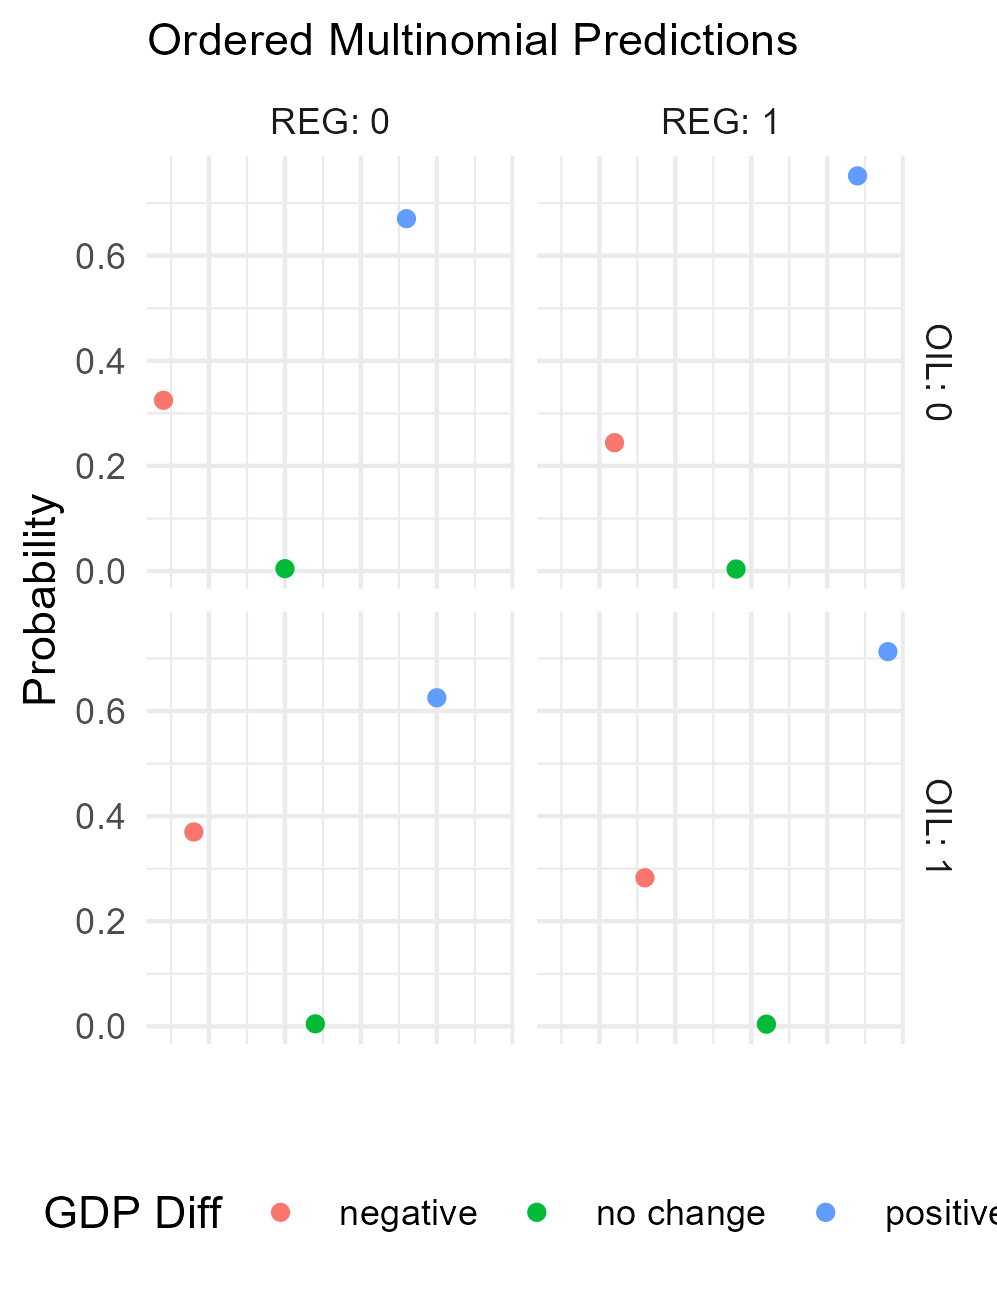
\includegraphics[width=0.7\textwidth]{graphics/pred_ord.png}
	  \caption{GDP Diff - ordered multinomial predictions}
	  \label{fig:pred:ord}
	\end{figure}

  The model predictions for the individual GDP difference categories are give in Table~\ref{tbl:parallel}  The proportional-odds assumption does not appear to hold for this regression i.e. the coefficients are not consistent (coef for \texttt{OIL} goes from -0.04 to 0.05 to -0.01).

    \lstinputlisting[language=R, firstline=321, lastline=327]{PS3_ImeldaFinn.R}
  
  \input{tables/q1_parallel_lines.tex}

\end{enumerate}

\paragraph[cutoffs]
  The cutoff point affects the results.  For example, changing the cutoff to split the data into 3 equal-length sections changes the coefficients and the confusion matrices. The resulting models aren't more accurate, because they reduce the number of true positive predictions for \emph{positive} without increasing the true predictions for the other 2 categories enough to compensate.  They also have higher deviance.  They could be refined to better categorise/predict the data.
  
  \begin{lstlisting}
    cutoffs:  <=14, 14-283,   >=283
---------------------------------------------------------------------
Multinomial model    
                         Dependent variable:     
                  ----------------------------
                     negative      positive   
                       (1)            (2)     
----------------------------------------------
REG                  0.184**       1.365***   
                     (0.088)        (0.087)   
                                              
OIL                  0.428***      0.641***   
                     (0.139)        (0.145)   
                                              
Constant             -0.091*       -0.649***  
                     (0.051)        (0.059)  
  
deviance: 7850.215

confusion matrix:
pred_m_all  no change negative positive
  no change       799      747      393
  negative         82       99      107
  positive        353      395      746

---------------------------------------------------------------------
Ordered Model
                Dependent variable:    
             ---------------------------
                        odiff           
----------------------------------------
REG                   0.930***          
                       (0.064)          
                                        
OIL                     0.120           
                       (0.105)          

deviance: 7691.950

confusion matrix:
pred_o_all  negative no change positive
  negative       846       881      500
  no change        0         0        0
  positive       395       353      746                   
---------------------------------------------------------------------
\end{lstlisting}
  
\begin{comment}
\end{comment}

\clearpage

%# Fri Feb 10 18:04:12 2023 ------------------------------

\section*{Question 2} 
\vspace{.25cm}

\noindent Consider the data set \texttt{MexicoMuniData.csv}, which includes municipal-level information from Mexico. The outcome of interest is the number of times the winning PAN presidential candidate in 2006 (\texttt{PAN.visits.06}) visited a district leading up to the 2009 federal elections, which is a count. Our main predictor of interest is whether the district was highly contested, or whether it was not (the PAN or their opponents have electoral security) in the previous federal elections during 2000 (\texttt{competitive.district}), which is binary (1=close/swing district, 0=``safe seat"). We also include \texttt{marginality.06} (a measure of poverty) and \texttt{PAN.governor.06} (a dummy for whether the state has a PAN-affiliated governor) as additional control variables. 

\begin{comment}
  \begin{figure}[!htbp]
	  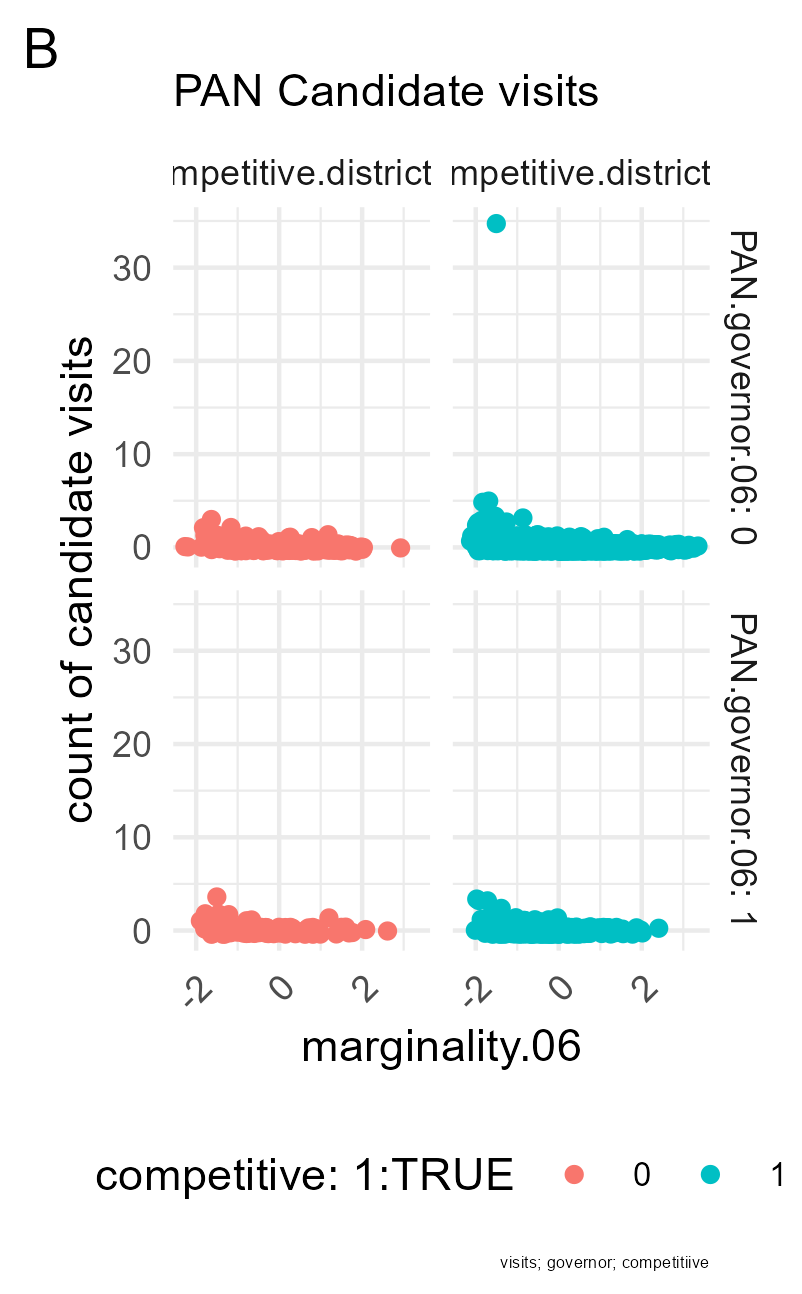
\includegraphics[width=0.7\textwidth]{graphics/mex_jitter.png}
	  \caption{Visit count data (jittered)}
	  \label{fig:mex:jitter}
	\end{figure}
%	\clearpage
\end{comment}

  \begin{figure}[!htbp]
	  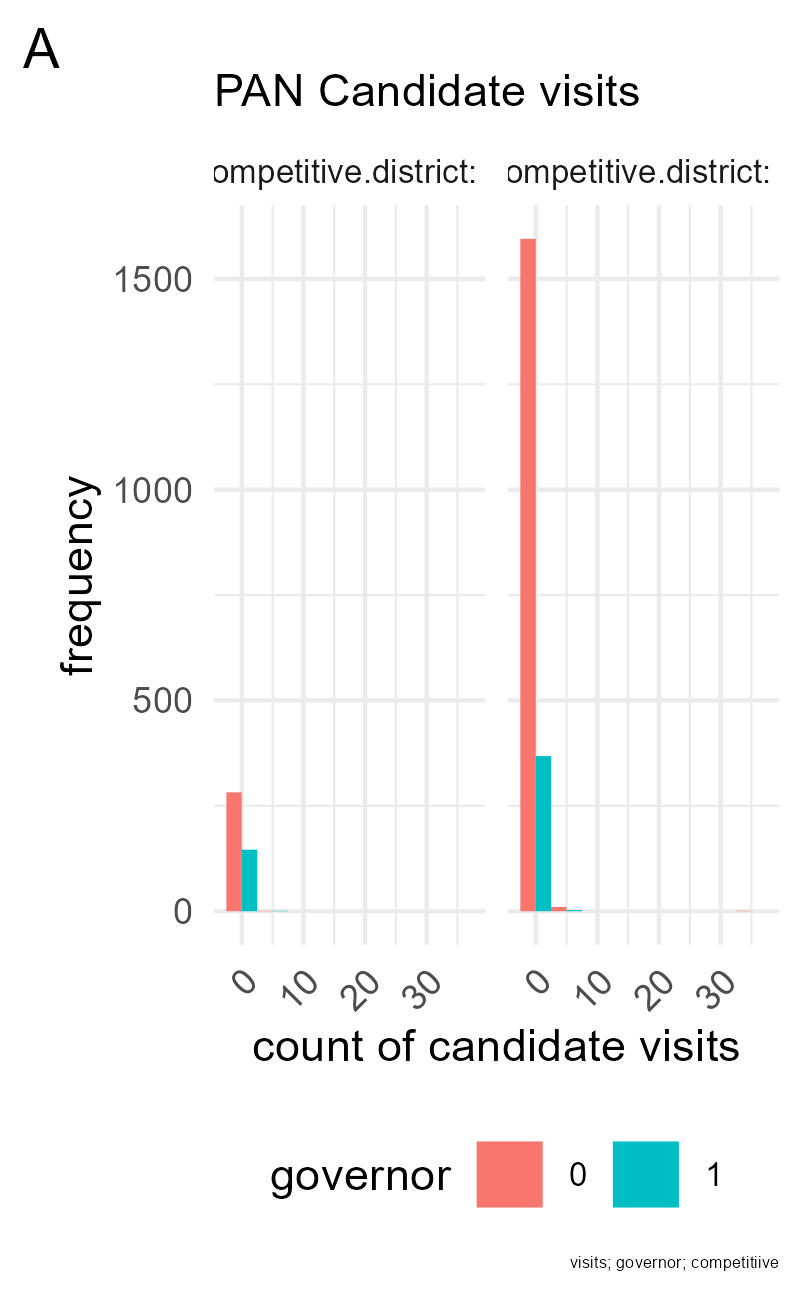
\includegraphics[width=0.7\textwidth,height=0.5\textheight]{graphics/mex_hist.png}
%	\end{figure}

%  \begin{figure}[!htbp]
%	  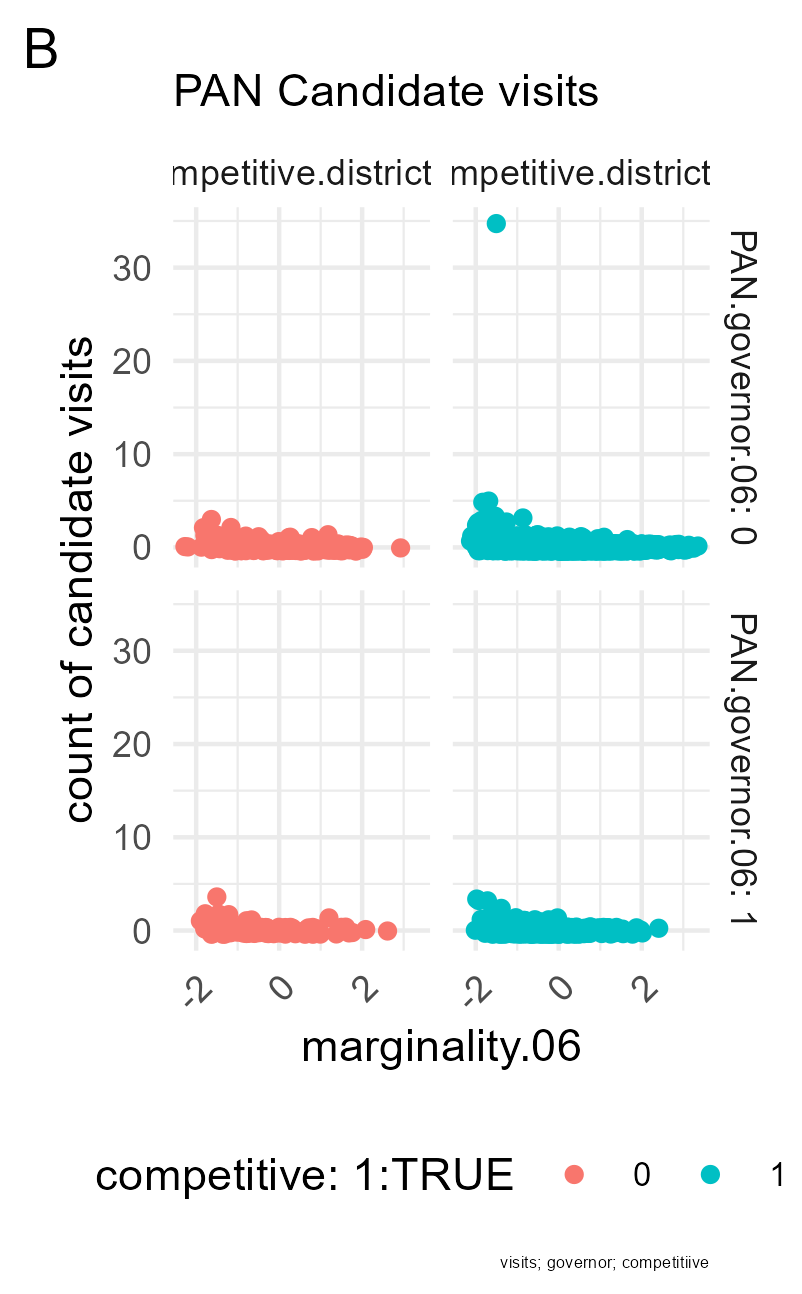
\includegraphics[width=0.7\textwidth]{graphics/mex_jitter.png}
	  \caption{Presidential candidate visits}
	  \label{fig:mex}
	\end{figure}
%	\clearpage
    \lstinputlisting[language=R, firstline=461, lastline=461]{PS3_ImeldaFinn.R}

\begin{enumerate}
	\item [(a)] A Poisson regression model was run because the outcome is a count variable, to consider whether there is evidence that PAN presidential candidates visit swing districts more?  The model output is in Table~\ref{tbl:poisson}. \texttt{competitive.district} coefficient is -0.081, but it is not a significant predictor for number of visits.
	% Provide a test statistic and p-value. 
    \lstinputlisting[language=R, firstline=525, lastline=526]{PS3_ImeldaFinn.R}

  A poisson model was run to get the regression coefficients.  
    
% Table created by stargazer v.5.2.3 by Marek Hlavac, Social Policy Institute. E-mail: marek.hlavac at gmail.com
% Date and time: Wed, Mar 22, 2023 - 00:04:38
\begin{table}[!htbp] \centering 
  \caption{Poisson Model of candidate visit counts} 
  \label{tbl:poisson} 
\begin{tabular}{@{\extracolsep{5pt}}lc} 
\\[-1.8ex]\hline 
\hline \\[-1.8ex] 
 & \multicolumn{1}{c}{\textit{Dependent variable:}} \\ 
\cline{2-2} 
\\[-1.8ex] & PAN.visits.06 \\ 
\\[-1.8ex] & \textit{Poisson} \\ 
\hline \\[-1.8ex] 
 competitive.district & $-$0.081 \\ 
  & (0.171) \\ 
  & \\ 
 marginality.06 & $-$2.080$^{***}$ \\ 
  & (0.117) \\ 
  & \\ 
 PAN.governor.06 & $-$0.312$^{*}$ \\ 
  & (0.167) \\ 
  & \\ 
 Constant & $-$3.810$^{***}$ \\ 
  & (0.222) \\ 
  & \\ 
\hline \\[-1.8ex] 
Observations & 2,407 \\ 
Log Likelihood & $-$645.606 \\ 
Akaike Inf. Crit. & 1,299.213 \\ 
\hline 
\hline \\[-1.8ex] 
\textit{Note:}  & \multicolumn{1}{r}{$^{*}$p$<$0.1; $^{**}$p$<$0.05; $^{***}$p$<$0.01} \\ 
\end{tabular} 
\end{table}  


  \begin{figure}[!htbp]
	  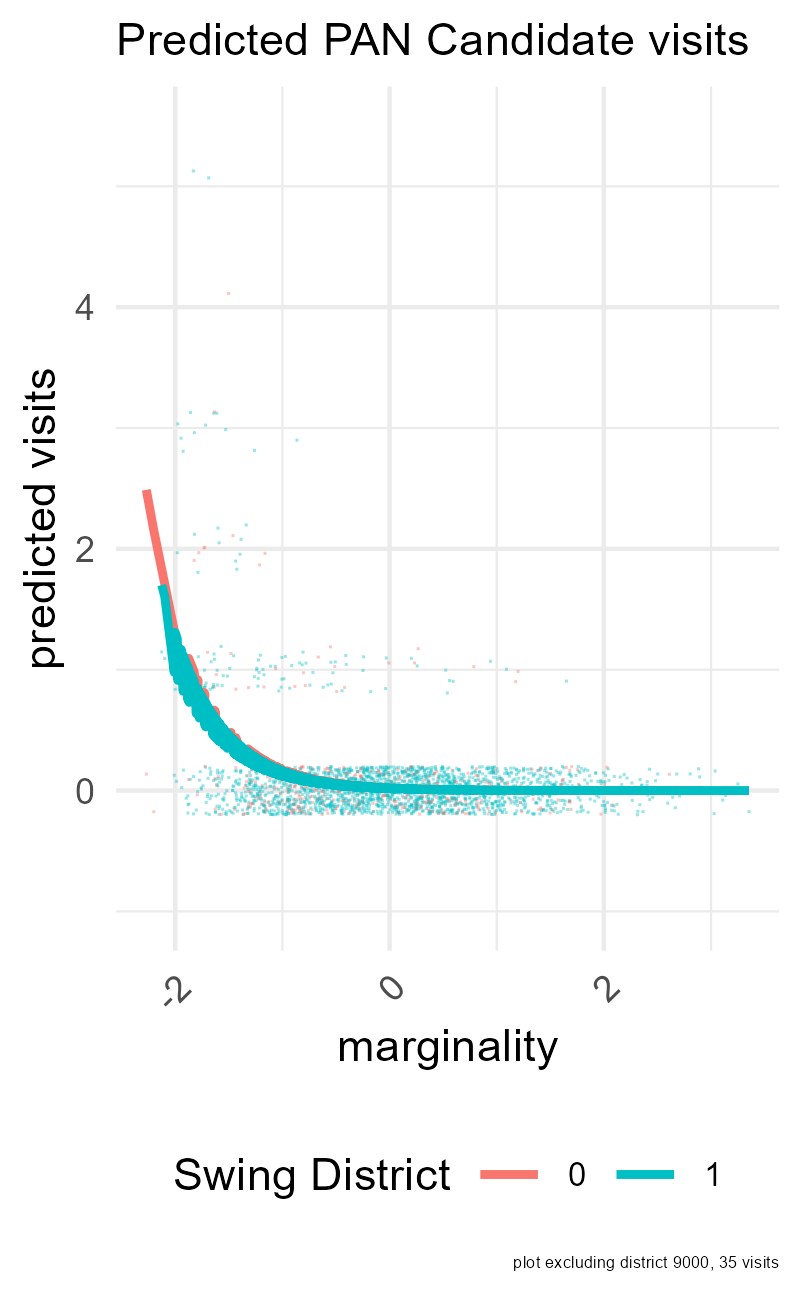
\includegraphics[width=0.7\textwidth,height=0.5\textheight]{graphics/mex_pred.png}
	  \caption{predicted presidential candidate visits}
	  \label{fig:mex:pred}
	\end{figure}

	\subsection*{Hypothesis Test}
    The summary results for the poisson model for the coefficients are:

\begin{lstlisting}
  Coefficients:
                       Estimate Std. Error z value Pr(>|z|)    
  (Intercept)          -3.81023    0.22209 -17.156   <2e-16 ***
  competitive.district -0.08135    0.17069  -0.477   0.6336    
  marginality.06       -2.08014    0.11734 -17.728   <2e-16 ***
  PAN.governor.06      -0.31158    0.16673  -1.869   0.0617 .  
\end{lstlisting}

	\begin{enumerate}[1.]
		\item $H_0$ PAN presidential candidate visits swing districts less than other districts  ($E(\lambda | competitive.district=1) <E(\lambda | competitive.district=0)$)
		\item $H_a$ candidates visit swing districts at least as many times other districts %(ie districts with \texttt{competitive.district} = 1 )
		\item the test statistic = $\beta_{competitive} / se_{competitive} =-0.08135/ 0.17069 = -0.477$ ($\sim N(0,1)$)
		\item the $\alpha$ value is 0.05, one-sided, left-tailed z-test 
		\item the \texttt{pvalue}  $p =  0.6833189 $ \footnote{pnorm(0.477)}
		%\item as \texttt{pvalue} is less than $\alpha$ we \textbf{reject} the null hypothesis
  \item as \texttt{pvalue} is greater than $\alpha$, we cannot reject the null hypothesis that closely contested districts receive fewer visits.

  Using R's \texttt{poisson.test}, the p-value is 0.8544, so we also reject the null hypothesis, i.e. there is not evidence to support the theory that presidential candidates visit swing districts more.
  
  \begin{lstlisting}[language=R]
  cd1 <-mexico$PAN.visits.06[mexico$competitive.district==1]
  cd0 <-mexico$PAN.visits.06[mexico$competitive.district==0]

  poisson.test(x=c(sum(cd1), sum(cd0)), T=c(length(cd1), length(cd0)),
             alternative="greater", conf.level=0.95)

	Comparison of Poisson rates

  data:  c(sum(cd1), sum(cd0)) time base: c(length(cd1), length(cd0))
  count1 = 176, expected count1 = 181.52, p-value = 0.8544
  alternative hypothesis: true rate ratio is greater than 1
  95 percent confidence interval:
   0.6411102       Inf
  sample estimates:
  rate ratio 
  0.8506716 
 \end{lstlisting}
  \begin{comment}  

  The confidence interval for \texttt{competitive.district} (at $\alpha=0.05$) does not include 0. %!!! not checking 2 tailed
  \end{comment}

	\end{enumerate}

	\item [(b)]  \texttt{marginality.06} and \texttt{PAN.governor.06} coefficients.
  \begin{lstlisting}[language=R]
    > lo_cis<-cbind(logOdds = coef(mexico_poisson), confint(mexico_poisson))
    Waiting for profiling to be done...

    # Coefficients and confidence intervals
                             logOdds      2.5 %       97.5 %
    (Intercept)          -3.81023498 -4.2606981 -3.389583340
    competitive.district -0.08135181 -0.4063661  0.264275617
    marginality.06       -2.08014361 -2.3151624 -1.855053854
    PAN.governor.06      -0.31157887 -0.6484827  0.006518468

    > exp(lo_cis) 
                          exp(beta) 2.5 % 97.5 %
    (Intercept)               0.022 0.014  0.034
    competitive.district      0.922 0.666  1.302
    marginality.06            0.125 0.099  0.156
    PAN.governor.06           0.732 0.523  1.007
  \end{lstlisting}

	
%An increase of 1 year in age increases expected number
%of ... by a multiplicative factor of e^0.06859 ~ 1:07
  \texttt{marginality.06} is the only coefficient which is significant at $\alpha=0.01$; \texttt{PAN.governor.06} is significant at $\alpha=0.1$.
  
	The coefficient for \texttt{marginality.06} is -2.08 ($CI_{0.05} = -2.315, -1.855$).  This means that, keeping all else constant, we expect a decrease of 2.08 in log count for a one-unit increase in \texttt{marginality.06}, i.e. if \texttt{marginality.06} increases by 1, we expect the estimated mean number of visits to decrease by 87.5\% (multiply previous expected count by $e^{-2.08}=0.125$).  Districts with higher marginality receive fewer visits.
	
	The coefficient for \texttt{PAN.governor.06} is -0.312, which means that if \texttt{PAN.governor.06} switches from 0 to 1, keeping all other variables constant, we expect an decrease in log count of 0.312.  If \texttt{PAN.governor.06} changes from 0 to 1, we expect the estimated mean number of visits to decrease by 26.8\% (ie multiply previous expected count by 0.732).  Districts with a PAN governor are expected to receive fewer visits from PAN candidates.  Note:  $CI_{0.05} = -0.648, 0.007$, which includes 0.  The test results suggest that having a PAN governor is not a significant predictor for the number of candidate visits.

	\item [(c)] The estimated mean number of visits from the winning PAN presidential candidate for a hypothetical district that was competitive (\texttt{competitive.district}=1), had an average poverty level (\texttt{marginality.06} = 0), and a PAN governor (\texttt{PAN.governor.06}=1).

  \begin{lstlisting}[language=R]
    mex_pred_data <- data.frame(competitive.district = 1, 
                            marginality.06=0,
                            PAN.governor.06=1)
    pred_mex <- cbind(predict(mexico_poisson,
                          mex_pred_data,
                          type= "response", se.fit =TRUE),
                  mex_pred_data)
    # create lower and upper bounds for CIs
    pred_mex$lowerBound <- pred_mex$fit - 1.96 * pred_mex$se.fit
    pred_mex$upperBound <- pred_mex$fit + 1.96 * pred_mex$se.fit

    round(pred_mex,3)


     fit se.fit residual.scale competitive.district marginality.06
1 0.015  0.003              1                    1              0
  PAN.governor.06 lowerBound upperBound
1               1      0.009      0.021

  
  \end{lstlisting}
  $\lambda = e^{\beta_0 + \beta_{competitive}\times competitive +  \beta_{marginality}\times marginality +  \beta_{governor}\times governor }$
  
  $= e^{ -3.810  - 0.081\times 1 +  -2.080\times 0 +  -0.312\times 1 } = e^{-4.203} = 0.015$  (The mean visits is 0.092, the median is 0.)
	
	The estimated mean number of visits, in the time frame, by the winning PAN presidential candidate to a district which was a swing state, with average poverty (=0) and a PAN governor is 0.015. 
\clearpage

  \item[]
  \textbf{Validation}
  There are 2,272 zero count values in our dataset.
 
  \begin{lstlisting}[language=R]
  dispersiontest(mexico_poisson)

  	Overdispersion test

  data:  mexico_poisson
  z = 1.0668, p-value = 0.143
  alternative hypothesis: true dispersion is greater than 1
  sample estimates:
  dispersion 
     2.09834 
\end{lstlisting}

  %The p-value is 0.143, we cannot reject the null hypothesis. A standard poisson distribution may not be a good fit.  
    A zero-inflated poisson model was run for comparison, the only coefficient with a significant deviance is the \texttt{marginality.06}, where an increase of 1 unit in marginality corresponds to a increase in log-odds of a 0 count value of 0.872(Table~\ref{tbl:zip:pois}).  The zero-inflated poisson changes the value of the coefficients, but doesn't change their statistical significance.
  
  
% Table created by stargazer v.5.2.3 by Marek Hlavac, Social Policy Institute. E-mail: marek.hlavac at gmail.com
% Date and time: Wed, Mar 22, 2023 - 20:51:31
\begin{table}[!htbp] \centering 
  \caption{Zero-inflation model} 
  \label{tbl:zip} 
\begin{tabular}{@{\extracolsep{5pt}}lc} 
\\[-1.8ex]\hline 
\hline \\[-1.8ex] 
 & \multicolumn{1}{c}{\textit{Dependent variable:}} \\ 
\cline{2-2} 
\\[-1.8ex] & PAN.visits.06 \\ 
\\[-1.8ex] & \textit{zero-inflated} \\ 
 & \textit{count data} \\ 
\hline \\[-1.8ex] 
 competitive.district & 0.900$^{*}$ \\ 
  & (0.511) \\ 
  & \\ 
 marginality.06 & 0.872$^{***}$ \\ 
  & (0.302) \\ 
  & \\ 
 PAN.governor.06 & $-$0.175 \\ 
  & (0.412) \\ 
  & \\ 
 Constant & 1.272$^{*}$ \\ 
  & (0.675) \\ 
  & \\ 
\hline \\[-1.8ex] 
Observations & 2,407 \\ 
Log Likelihood & $-$600.386 \\ 
\hline 
\hline \\[-1.8ex] 
\textit{Note:}  & \multicolumn{1}{r}{$^{*}$p$<$0.1; $^{**}$p$<$0.05; $^{***}$p$<$0.01} \\ 
\end{tabular} 
\end{table}  

% Table created by stargazer v.5.2.3 by Marek Hlavac, Social Policy Institute. E-mail: marek.hlavac at gmail.com
% Date and time: Wed, Mar 22, 2023 - 20:51:32
\begin{table}[!htbp] \centering 
  \caption{Zero Infl Poisson vs Poisson Model} 
  \label{tbl:zip:pois} 
\begin{tabular}{@{\extracolsep{5pt}}lcc} 
\\[-1.8ex]\hline 
\hline \\[-1.8ex] 
 & \multicolumn{2}{c}{\textit{Dependent variable:}} \\ 
\cline{2-3} 
\\[-1.8ex] & \multicolumn{2}{c}{PAN.visits.06} \\ 
\\[-1.8ex] & \textit{zero-inflated} & \textit{Poisson} \\ 
 & \textit{count data} & \textit{} \\ 
\hline \\[-1.8ex] 
 competitive.district & 0.402 & $-$0.081 \\ 
  & (0.312) & (0.171) \\ 
  & & \\ 
 marginality.06 & $-$1.240$^{***}$ & $-$2.080$^{***}$ \\ 
  & (0.261) & (0.117) \\ 
  & & \\ 
 PAN.governor.06 & $-$0.470$^{*}$ & $-$0.312$^{*}$ \\ 
  & (0.271) & (0.167) \\ 
  & & \\ 
 Constant & $-$1.914$^{***}$ & $-$3.810$^{***}$ \\ 
  & (0.498) & (0.222) \\ 
  & & \\ 
\hline \\[-1.8ex] 
Observations & 2,407 & 2,407 \\ 
Log Likelihood & $-$600.386 & $-$645.606 \\ 
Akaike Inf. Crit. &  & 1,299.213 \\ 
\hline 
\hline \\[-1.8ex] 
\textit{Note:}  & \multicolumn{2}{r}{$^{*}$p$<$0.1; $^{**}$p$<$0.05; $^{***}$p$<$0.01} \\ 
\end{tabular} 
\end{table}  

\begin{lstlisting}
  anova(mexico_poisson, zeroinfl_poisson, test = "Chi")
  Analysis of Deviance Table

  Model: poisson, link: log

  Response: PAN.visits.06

  Terms added sequentially (first to last)


                         Df Deviance Resid. Df Resid. Dev Pr(>Chi)    
    NULL                                  2406    1473.87             
    competitive.district  1     0.91      2405    1472.96  0.34078    
    marginality.06        1   478.03      2404     994.93  < 2e-16 ***
    PAN.governor.06       1     3.68      2403     991.25  0.05502 
\end{lstlisting}

  There is one outlier with visits = 35; predicted visits based on the model are 0.467.  Excluding that district (ie assuming it's bad data) would lead to changes in the model, but would only change the prediction in c) from 0.015 to  0.016.
  
  \begin{lstlisting}
                              PAN.visits.06        
                outlier removed       default     
-------------------------------------------------
competitive.district     -0.261        -0.081    
                        (0.176)        (0.171)   
marginality.06         -1.954***      -2.080***  
                        (0.124)        (0.117)   
PAN.governor.06          -0.129        -0.312*   
                        (0.172)        (0.167)   
Constant               -3.727***      -3.810***  
                        (0.227)        (0.222)   
-------------------------------------------------
Observations             2,406          2,407    
Log Likelihood          -521.651      -645.606   
Akaike Inf. Crit.      1,051.301      1,299.213  
  \end{lstlisting}

\end{enumerate}

\begin{comment}  
  \begin{lstlisting}
  mexico_null <- glm(PAN.visits.06 ~ 1, data= mexico, family =poisson )
  > anova(mexico_null, mexico_poisson, test = "Chisq")
  Analysis of Deviance Table

  Model 1: PAN.visits.06 ~ 1
  Model 2: PAN.visits.06 ~ competitive.district + marginality.06 + PAN.governor.06
    Resid. Df Resid. Dev Df Deviance  Pr(>Chi)    
  1      2406    1473.87                          
  2      2403     991.25  3   482.62 < 2.2e-16 ***
\end{lstlisting}
  \end{comment]


\begin{comment}
  \begin{figure}[!htbp]
	  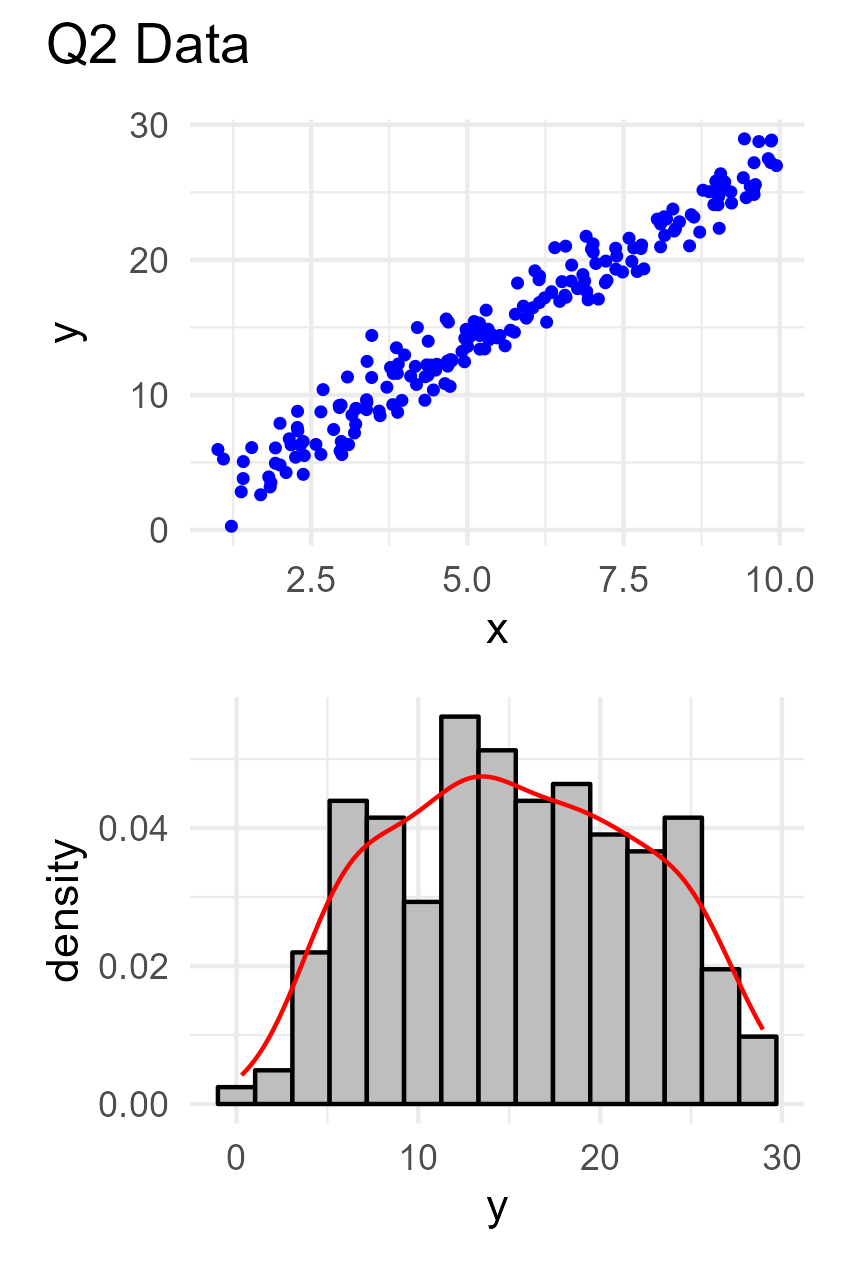
\includegraphics[width=0.85\textwidth]{graphics/q2_data.png}
	  \caption{Q2 Data}
	  \label{fig:mle:data}
	\end{figure}

  \begin{figure}[!htbp]
	  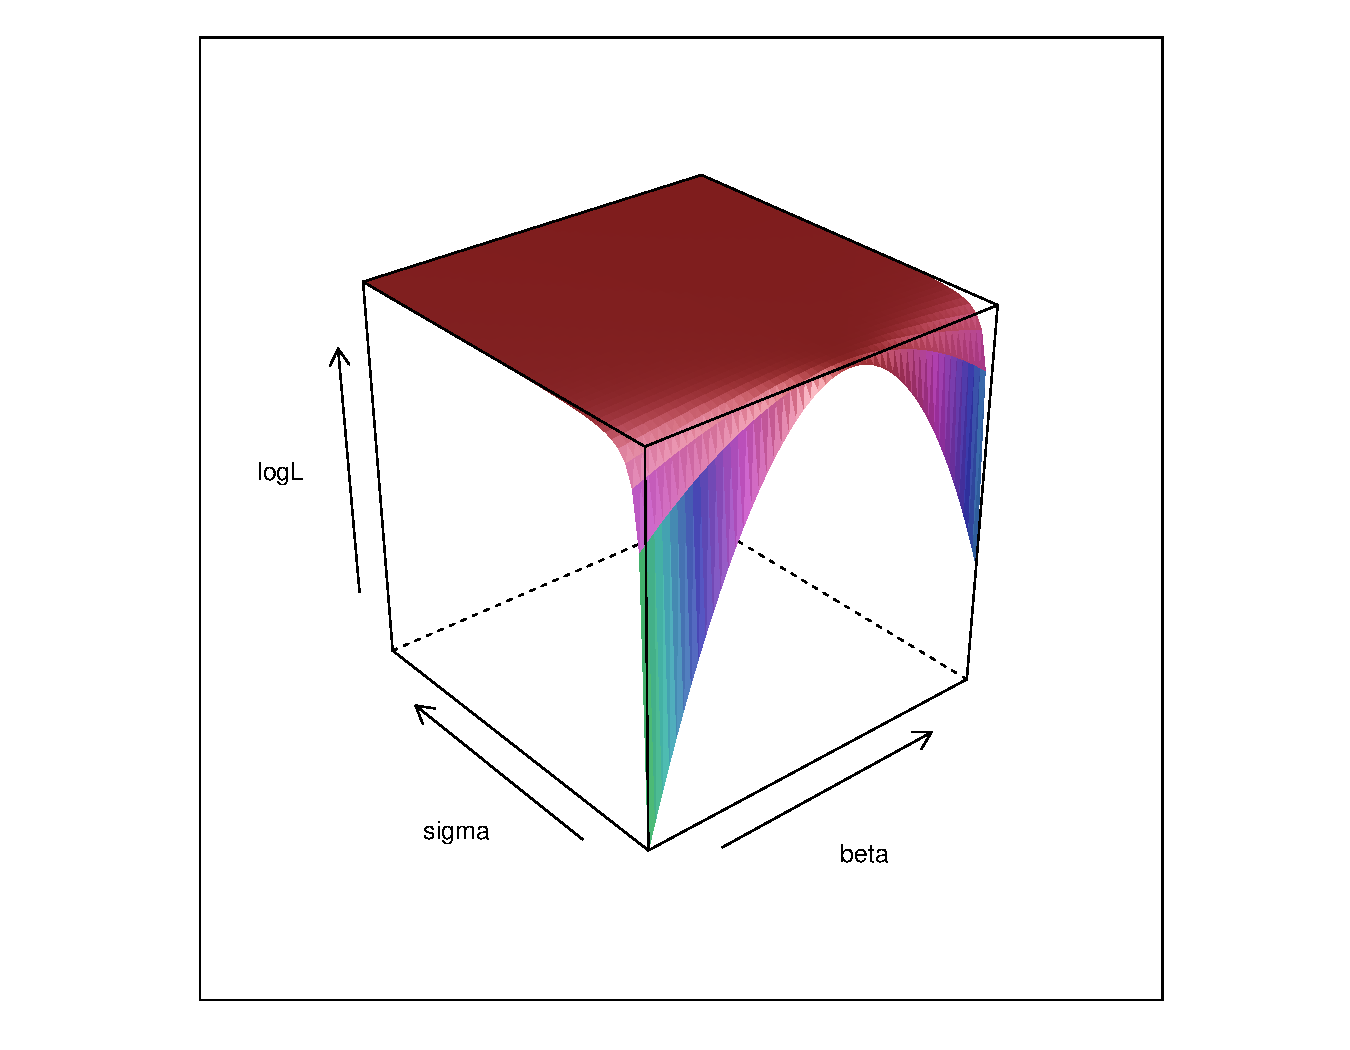
\includegraphics[width=0.7\textwidth]{graphics/wireframe.pdf}
	  \caption{mle surface}
	  \label{fig:surface}
	\end{figure}
  \begin{figure}[!htbp]
	  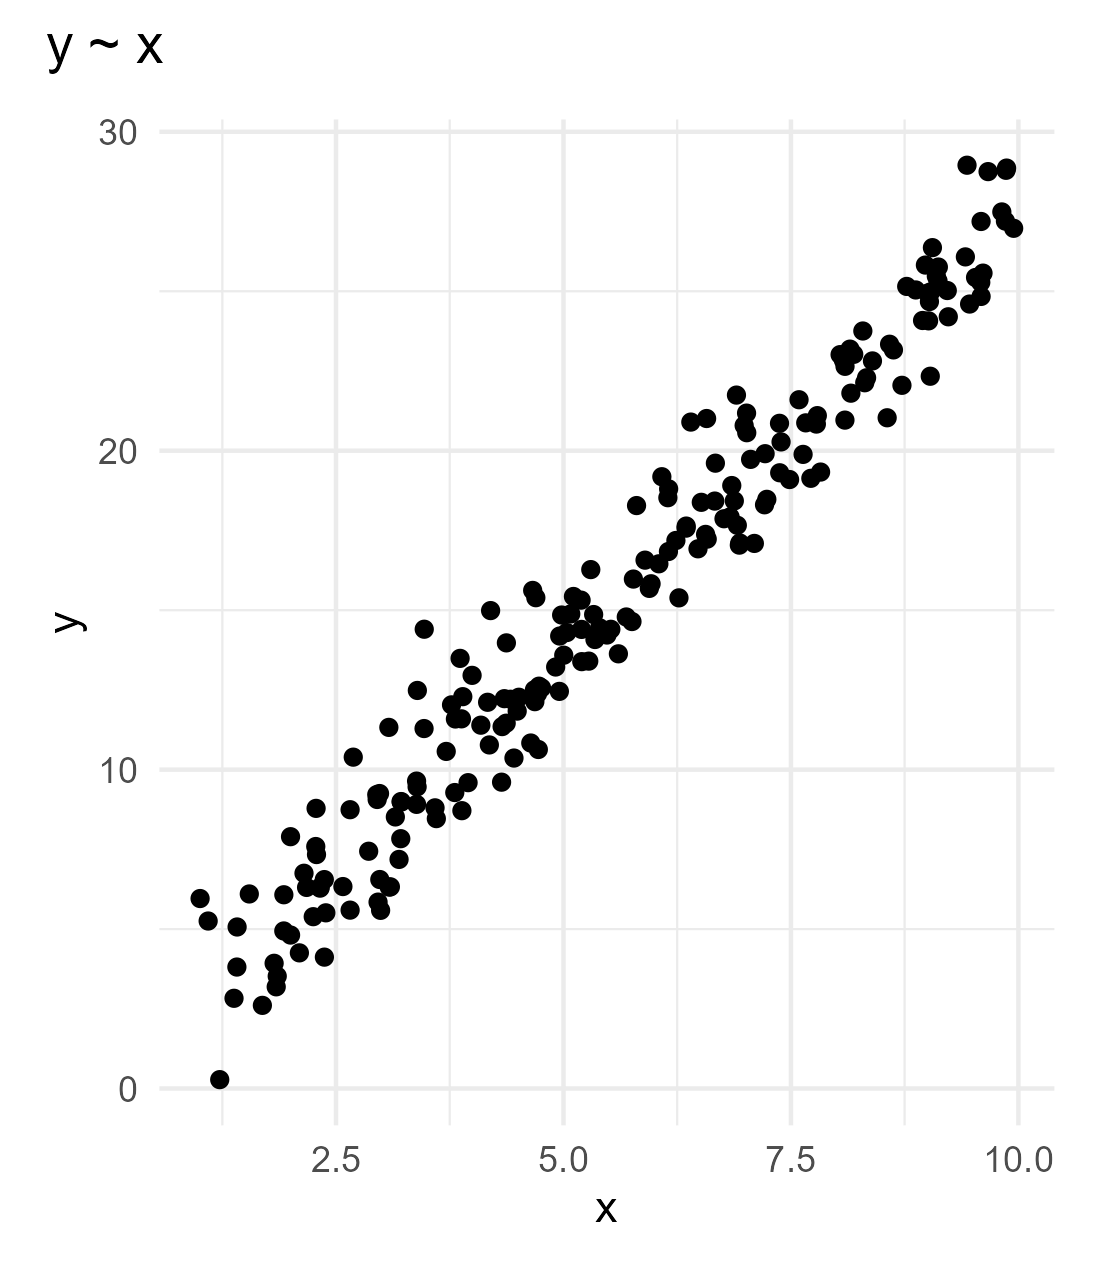
\includegraphics[width=0.7\textwidth]{graphics/q2_xy.png}
	  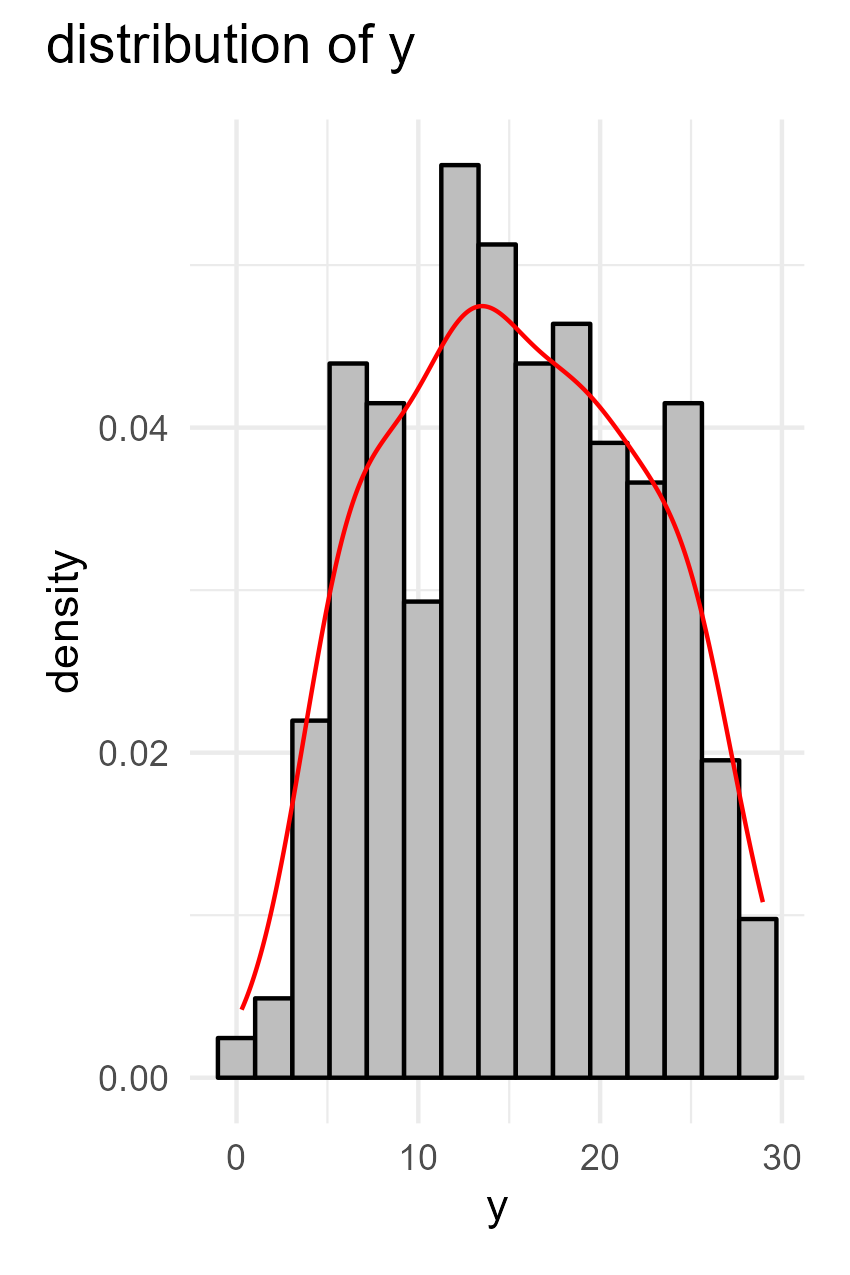
\includegraphics[width=0.7\textwidth]{graphics/q2_hist.png}
	  \caption{Q2 Data}
	  \label{fig:mle}
	\end{figure}
\end{comment}

\begin{comment}
	\clearpage

\lstinputlisting[language=R, firstline=3,lastline=3]{PS3_ImeldaFinn.R}

	The prediction equation is: $y = 0.1398324 + 2.7265559 \times x$.

	$\hat y =  0.13983  (\theta)  +  5.55753  (\bar{x}) *  2.72656  (\beta) =  15.29274$

	$\bar y = 15.29289$
\end{comment}

%https://www.sascha-frank.com/Faq/tables_three.html
%http://www.sthda.com/english/wiki/ggplot2-facet-split-a-plot-into-a-matrix-of-panels#facet-labels

\end{document}
